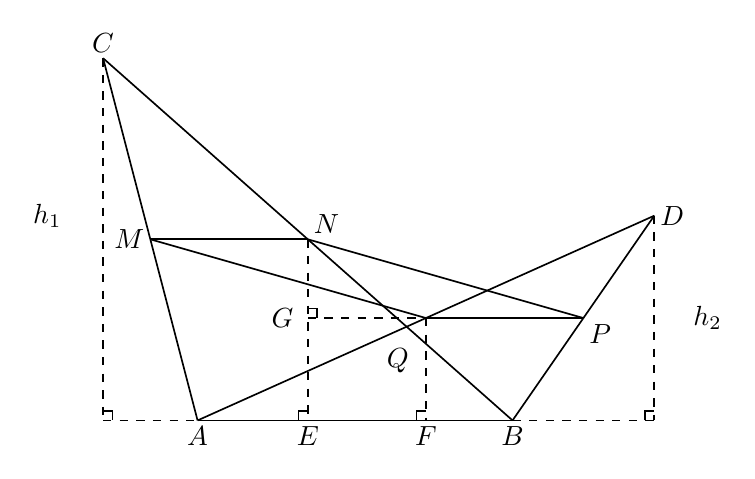
\begin{tikzpicture}[x=1cm,y=1cm,font=\normalsize,
 geometry edge/.style={solid,line width=.6pt},
 geometry mark/.style={solid,line width=.6pt},
 geometry label/.style={font=\normalsize,inner sep=2pt}]
\coordinate (A) at (1.5,0.0);
\coordinate (B) at (5.5,0.0);
\coordinate (C) at (0.3,4.6);
\coordinate (D) at (7.3,2.6);
\coordinate (M) at (0.9,2.3);
\coordinate (N) at (2.9,2.3);
\coordinate (P) at (6.4,1.3);
\coordinate (Q) at (4.4,1.3);
\coordinate (E) at (2.9,0.0);
\coordinate (F) at (4.4,0.0);
\coordinate (HC) at (0.3,0.0);
\coordinate (HD) at (7.3,0.0);
\coordinate (G) at (2.9,1.3);
\coordinate (LH1) at (-0.15,2.6);
\coordinate (LH2) at (7.72,1.3);
\draw[geometry edge] (A)--(B);
\draw[geometry edge] (A)--(M);
\draw[geometry edge] (M)--(C);
\draw[geometry edge] (B)--(N);
\draw[geometry edge] (N)--(C);
\draw[geometry edge] (A)--(Q);
\draw[geometry edge] (Q)--(D);
\draw[geometry edge] (B)--(P);
\draw[geometry edge] (P)--(D);
\draw[geometry edge] (M)--(N);
\draw[geometry edge] (N)--(P);
\draw[geometry edge] (P)--(Q);
\draw[geometry edge] (Q)--(M);
\draw[geometry edge,dashed] (C)--(HC);
\draw[geometry edge,dashed] (D)--(HD);
\draw[geometry edge,dashed] (N)--(E);
\draw[geometry edge,dashed] (Q)--(F);
\draw[geometry edge,dashed] (G)--(Q);
\draw[geometry edge,dashed] (HC)--(A);
\draw[geometry edge,dashed] (B)--(HD);
\draw[geometry mark] (2.78,0) -- (2.78,0.12) -- (2.9,0.12);
\draw[geometry mark] (4.28,0) -- (4.28,0.12) -- (4.4,0.12);
\draw[geometry mark] (7.18,0) -- (7.18,0.12) -- (7.3,0.12);
\node[geometry label,below] at (A) {$A$};
\node[geometry label,below] at (B) {$B$};
\node[geometry label,above] at (C) {$C$};
\node[geometry label,right] at (D) {$D$};
\node[geometry label,left] at (M) {$M$};
\node[geometry label,above right] at (N) {$N$};
\node[geometry label,below right] at (P) {$P$};
\node[geometry label,below left,xshift=-4pt,yshift=-9pt] at (Q) {$Q$};
\node[geometry label,below] at (E) {$E$};
\node[geometry label,below] at (F) {$F$};
\node[geometry label,left] at (LH1) {$h_1$};
\node[geometry label,right] at (LH2) {$h_2$};
\draw[geometry mark] (.3,.12)--(.42,.12)--(.42,0);
\draw[geometry mark] (2.9,1.42)--(3.02,1.42)--(3.02,1.3);
\node[geometry label,left,xshift=-3pt] at (G) {$G$};
\end{tikzpicture}
